\newpage
\section{Auswertung}
Im folgenden Kapitel werden die aufgenommenen Messwerte ausgewertet und die Ergebnisse 
diskutiert.\\
\textit{Hinweis} beim aufzeichnen der Messwerte, ist ab dem invertierenden Integrator
ein unbekannter Fehler im Experiment aufgetreten. Dieser ist dafür verantwortlich, dass
unsere Messwerte ab diesem Zeitpunkt unbrauchbar geworden sind.
Damit dennoch die wesentlichen Zusammenhänge und Ziele des Experiments gezeigt werden können,
sind Messwerte von zwei unterschiedlichen Gruppen für die weitere Auswertung herangezogen worden.
Die Benutzung sowie die Quellen der Messwerte,
ist in diesem Abschnitt an unterschiedlichen Stellen kenntlich gemacht.

\section{Der invertierende Verstärker / Linearverstärker}
\subsection{Untersuchung der Verstärkung}
Im ersten Teil des Versuches wird das Frequenzabhängige Verhalten der Verstärkung untersucht.
Hierzu wird die Ausgangsspannung in Abhängigkeit der Frequenz über mehrere Dekaden gemessen 
und die Verstärkung in einem doppellogarithmischen Plot aufgetragen aufgetragen.
Es sind insgesamt drei unterschiedliche Verstärkungen untersucht worden.
Die Plots sind sind in \autoref{fig:Linearverstaerker} dargestellt.
Per linearer Regression
\begin{equation*}
    f(x) = mx+b,
\end{equation*}
lassen sich die Verstärkung, die Grenzfrequenz und das Bandbreitenprodukt bestimmen.
Im Plot schwarz markierte Messwerte werden als Ausreißer betrachtet 
und fließen nicht in die Berechnungen ein.
Die errechneten Parameter sind in \autoref{tab:params} dargestellt.
Hierbei ist $V_\text{theo}$ die theoretische Verstärkung, berechnet anhand des gewählten 
Widerstandsverhältnisses, $V_\text{b}$ die gemessene Verstärkung, $f_\text{gr}$ die 
gemessene Grenzfrequenz und $GBP$ das aus den Messwerten 
(vgl. Anhang \ref{sub:Messwerte des Linarverstärkers}) errechnete Bandbreitenprodukt.
\input{build/tabParameter_Linearverstärker.tex}
\FloatBarrier
Betrachtet man die unterschiedlichen Graphen so lässt sich erkennen, dass
die jeweiligen Verstärkungen bei niedrigen Frequenzen in guter Näherung konstant
bleiben. Mit steigender Frequenz fällt die Verstärkung im Plot linear ab.
Dies entspricht ganz den Erwartungen der vorrangestellten Theorie.
\begin{figure}
    \centering
    \begin{subfigure}[b]{0.45\textwidth}
        \centering
        \includegraphics[width=\textwidth]{build/a.pdf}
        \caption{Linearverstärker bei einer Verstärkung von 100. $R_1 = \SI{1}{\kilo\ohm}$,
        $R_2 = \SI{100}{\kilo\ohm}$ }
        \label{fig:a}
    \end{subfigure}
    \hfill
    \begin{subfigure}[b]{0.45\textwidth}
        \centering
        \includegraphics[width=\textwidth]{build/b.pdf}
        \caption{Linearverstärker bei einer Verstärkung von 10. $R_1 = \SI{10}{\kilo\ohm}$,
        $R_2 = \SI{100}{\kilo\ohm}$ }
        \label{fig:b}
    \end{subfigure}
    \newline
    \newline    
    \newline    
    \newline    
    \begin{subfigure}[b]{0.45\textwidth}
        \centering
        \includegraphics[width=\textwidth]{build/c.pdf}
        \caption{Linearverstärker bei einer Verstärkung von 1000. $R_1 = \SI{100}{\ohm}$,
        $R_2 = \SI{100}{\kilo\ohm}$ }
        \label{fig:c}
    \end{subfigure}
       \caption{Aufgenommene Graphen bei unterschiedlichen Verstärkungsfaktoren.}
       \label{fig:Linearverstaerker}
\end{figure}
\FloatBarrier

\subsection{Verhalten der Phasendifferenz bei steigender Frequenz}
Im nächsten Teil des Versuches wird die Phasenverschiebung von Ein- und Ausgangsspannung 
untersucht.
Dazu wird die gemessene Phasendifferenz $\phi$ in Abhängigkeit der logarithmierten Frequenz $f$
aufgetragen.
Die Plots sind sind in \autoref{fig:phase} dargestellt.

Anhand der Plots ist erkennbar, dass mit steigender Frequenz die Phasendifferenz zwischen 
Ein- und Ausgangsspannung sinkt.
Da es sich bei der verwendeten Schaltung um einen invertierenden Verstärker handelt, beginnt 
der Phasenversatz bei $\SI{180}{\degree}$.

Des Weiteren lässt sich erkennen, dass je höher der Verstärkungsfaktor ist, desto früher
beginnt der Phasenversatz zu sinken. 
Bei der \autoref{fig:phase_1000} wurden insgesamt 3 Messwerte rausgenommen und 
als Ausreißer identifiziert.

Betrachtet man insbesondere die \autoref{fig:phase_10} so ähnelt der Verlauf
des Graphen dem Verlauf eines Tiefpasses.
Bei einen Tiefpasses können niedrige Frequenzen passieren, wo hingegen hohe Frequenzen
unterdrückt werden.

\section{Der invertierende Integrator \cite{int_data}, \cite{int_picture}}
In diesem Abschnitt wird überprüft ob die Ausgangsspannung des Integrators sich proportional 
zur Frequenz verhält.
Dazu wird im Experiment die Ein- und Ausgangsspannung in Abhängigkeit der Frequenz gemessen.

Die Messdaten sind in \autoref{tab:integrator} zu finden. 
Wie bereits im obigen Hinweis erwähnt, handelt es sich bei den ausgewerteten Messwerten
um Fremddaten.

Im nächsten Schritt ist die Ausgangsspannung in Abhängigkeit der Frequenz in einem Plot
mit doppellogarithmischer Skala aufgetragen worden.
Dieser Plot ist in \autoref{fig:integrator} zu sehen.
Anschließend wird mit Hilfe der Regressionsfunktion
\begin{equation*}
    ln(f(x)) =  m\,ln(x) + b
\end{equation*}
der erste Bereich (bis ca. 1000\,Hz) gefittet.
Dadurch ist in \autoref{fig:integrator} der blaue Fit enstanden.

Anhand des blauen Fits ist erkennbar, dass sich die Ausgangsspannung antiproportional zu der Frequenz
verhält.
Dies ist genau was man aus der Theorie erwartet.

Wird allerdings der weitere Verlauf der Messwerte betrachtet so fällt auf, dass die 
Ausgangsspannung ab ca. 1000\,Hz wieder zu steigen beginnt. 
Dieser Effekt kann zum jetzigen Zeitpunkt noch nicht erklärt werden.
Im weiteren Verlauf beginnt diese aber wieder zu sinken (roter Fit), was der ursprünglichen 
Erwartung entspricht. 
Die beiden Steigungen der Fits sind nahezu gleich, was dafür spricht das der Abfall
auf dem selben Effekt beruht.
\begin{align*}
    m_\text{blau} &=  \SI{-0.87\pm0.05}{\volt\per\hertz}\\
    m_\text{rot} &=  \SI{-0.82\pm0.05}{\volt\per\hertz}
\end{align*}
\begin{figure}
    \centering
    \includegraphics[width=0.7\linewidth]{build/integrator.pdf}
    \caption{Ausgangsspannung in Abhängigkeit der Frequenz. $R = \SI{10}{\kilo\ohm}$,
        $C = \SI{100}{\nano\farad}$.}
    \label{fig:integrator}
\end{figure}
\FloatBarrier

Mit Hilfe der aufgebauten Integratorschaltung lassen sich verschiedene Eingangssignale 
integrieren. 
Im unserem Experiment werden die Integrationen einer Sinus-, einer Dreiecks- und einer Rechteckspannung 
untersucht.
Die Integrationen sind mit Hilfe eines Oszilloskops aufgezeichnet worden.
Daraus ergeben sich die Bilder in \autoref{fig:int}
\begin{figure}
    \centering
    \begin{subfigure}[b]{0.45\textwidth}
        \centering
        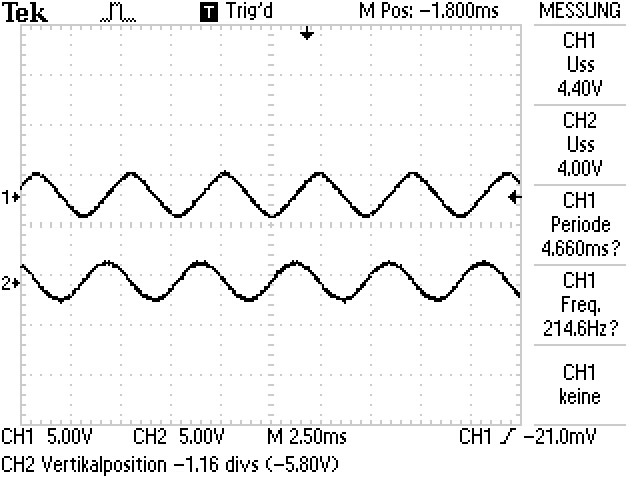
\includegraphics[width=\textwidth]{data_of_others_cuz_ours_suck/int/int_sinus.JPG}
        \caption{Oszillographische Darstellung einer integrierten Sinusspannung.
        Die integrierte Sinusspannung ist auf Channel 2 dargestellt und ist ein Kosinus.}
        \label{fig:int_sin}
    \end{subfigure}
    \hfill
    \begin{subfigure}[b]{0.45\textwidth}
        \centering
        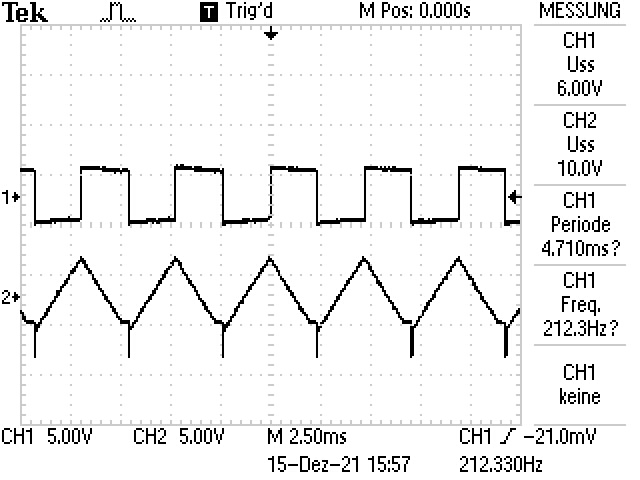
\includegraphics[width=\textwidth]{data_of_others_cuz_ours_suck/int/int_recht.JPG}
        \caption{Oszillographische Darstellung einer integrierten Rechteckspannung.
        Die integrierte Rechteckspannung ist auf Channel 2 dargestellt und ist eine Dreieckspannung.}
        \label{fig:int_recht}
    \end{subfigure}
    \newline
    \newline  
    \newline
    \newline  
    \newline  
    \begin{subfigure}{0.45\textwidth}
        \centering
        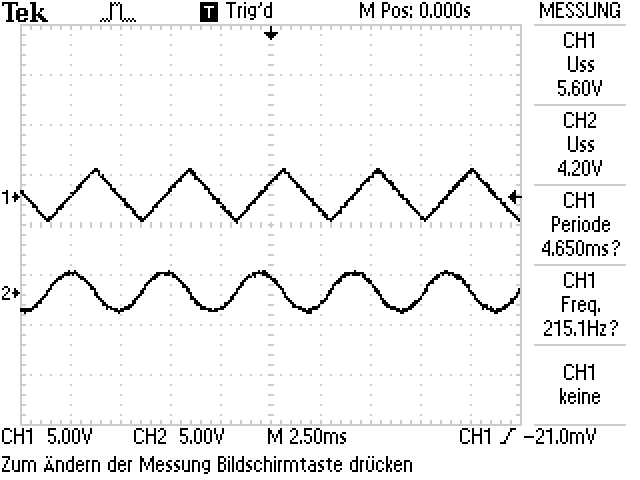
\includegraphics[width=\textwidth]{data_of_others_cuz_ours_suck/int/int_dreieck.JPG}
        \caption{Oszillographische Darstellung einer integrierten Dreieckspannung.
        Die integrierte Dreieckspannung ist auf Channel 2 dargestellt und zeigt einen Sinus.}
        \label{fig:int_drei}
    \end{subfigure}
       \caption{Ein- und Ausgangssignale eines invertierenden Integrators. Channel 1 zeigt
       das Eingangssignal. Channel 2 zeigt das integrierte Signal.}
       \label{fig:int}
\end{figure}
\FloatBarrier


\begin{figure}
    \centering
    \begin{subfigure}[b]{0.45\textwidth}
        \centering
        \includegraphics[width=\textwidth]{build/Phasenbeziehung_100.pdf}
        \caption{Phasenverschiebung zwischen Ein- und Ausgangsspannung bei einer Verstärkung von 100.}
        \label{fig:phase_100}
    \end{subfigure}
    \hfill
    \begin{subfigure}[b]{0.45\textwidth}
        \centering
        \includegraphics[width=\textwidth]{build/Phasenbeziehung_10.pdf}
        \caption{Phasenverschiebung zwischen Ein- und Ausgangsspannung bei einer Verstärkung von 10.}
        \label{fig:phase_10}
    \end{subfigure} 
    \newline
    \newline   
    \newline   
    \newline   
    \begin{subfigure}[b]{0.45\textwidth}
        \centering
        \includegraphics[width=\textwidth]{build/Phasenbeziehung_1000.pdf}
        \caption{Phasenverschiebung zwischen Ein- und Ausgangsspannung bei einer Verstärkung von 1000.}
        \label{fig:phase_1000}
    \end{subfigure}
       \caption{Aufgenommene Phasendifferenz unterschiedlichen Verstärkungsfaktoren.}
       \label{fig:phase}
\end{figure}
\FloatBarrier

\section{Der invertierende Differenzierer \cite{int_data}, \cite{int_picture}}
Analog zu dem invertierende Integrator, lassen sich die gleichen Betrachtungen 
für einen invertierende Differenzierer anstellen.
Der Plot welcher sich durch die Messwerte \autoref{tab:differenzierer} ergibt, ist in
\autoref{fig:differenzierer} zu sehen.
Anhand des Verlaufs der linearen Regression lässt sich feststellen, dass die Ausgangspannung
im Bereich von 100\,Hz bis ca. 4000\,Hz proportional zu der Frequenz der Eingangsspannung ist.
Dies stimmt mit den Erwartungen überein.

Wird die Frequenz der Eingangsspannung weiter erhöht beginnt die Ausgangspannung
wieder zu sinken.
Dies ist genau der umgekehrte experimentelle Befund, welcher beim invertierenden Integrator
ebenfalls aufgetreten ist.
Dieser kann zum jetzigen Zeitpunkt noch nicht erklärt werden.
\begin{figure}
    \centering
    \includegraphics[width=0.7\linewidth]{build/differenzierer.pdf}
    \caption{Ausgangsspannung in Abhängigkeit der Frequenz. $R = \SI{100}{\kilo\ohm}$,
        $C = \SI{22}{\nano\farad}$.}
    \label{fig:differenzierer}
\end{figure}
\FloatBarrier
Mit Hilfe der aufgebauten Differenziererschaltung lassen sich verschiedene Eingangssignale 
differenzierern. 
Hier werden ebenfalls eine Sinus-, einer Dreiecks- und einer Rechteckspannung 
untersucht.
Die Differenziationen sind mit Hilfe eines Oszilloskops aufgezeichnet worden.
Daraus ergeben sich die Bilder in \autoref{fig:diff}
\begin{figure}
    \centering
    \begin{subfigure}[b]{0.45\textwidth}
        \centering
        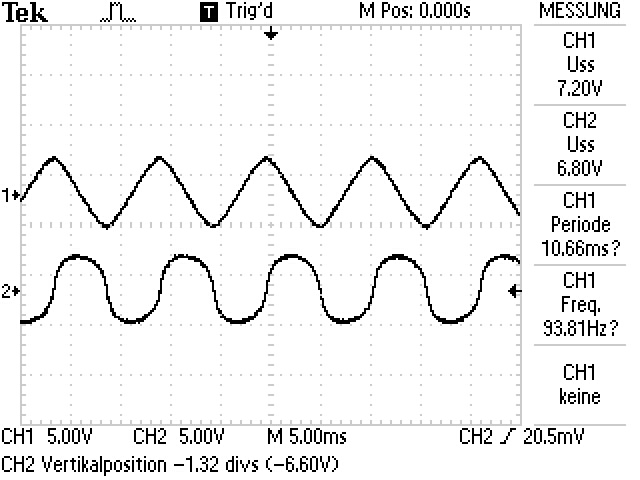
\includegraphics[width=\textwidth]{data_of_others_cuz_ours_suck/diff/diff_sin.JPG}
        \caption{Oszillographische Darstellung einer differenzierten Sinusspannung.
        Die differenzierte Sinusspannung ist auf Channel 2 dargestellt und ist ein Kosinus.}
        \label{fig:diff_sin}
    \end{subfigure}
    \hfill
    \begin{subfigure}[b]{0.45\textwidth}
        \centering
        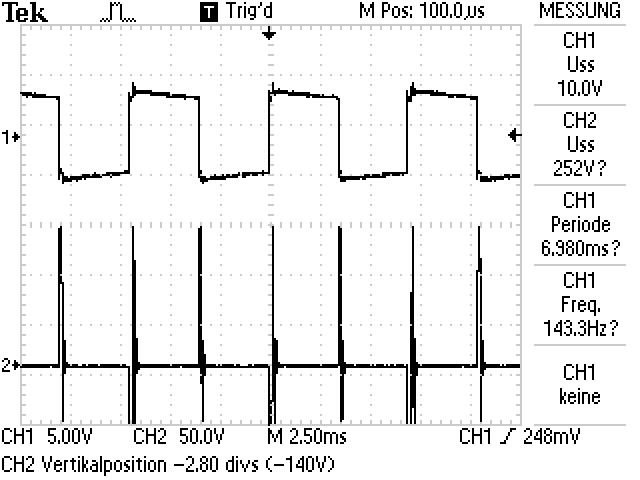
\includegraphics[width=\textwidth]{data_of_others_cuz_ours_suck/diff/diff_recht.JPG}
        \caption{Oszillographische Darstellung einer differenzierten Rechteckspannung.
        Die differenzierte Rechteckspannung ist auf Channel 2 dargestellt und sind Nadelpulse.}
        \label{fig:diff_recht}
    \end{subfigure}
    \newline
    \newline  
    \newline
    \newline  
    \newline  
    \begin{subfigure}{0.45\textwidth}
        \centering
        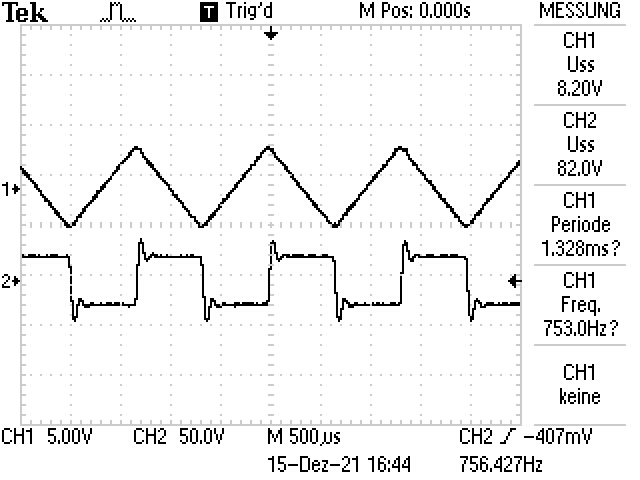
\includegraphics[width=\textwidth]{data_of_others_cuz_ours_suck/diff/diff dreieck.JPG}
        \caption{Oszillographische Darstellung einer differenzierten Dreieckspannung.
        Die differenzierte Dreieckspannung ist auf Channel 2 dargestellt und zeigt eine Rechteckspannung.}
        \label{fig:diff_drei}
    \end{subfigure}
       \caption{Ein- und Ausgangssignale eines invertierenden Differenzierers. Channel 1 zeigt
       das Eingangssignal. Channel 2 zeigt das differenzierte Signal.}
       \label{fig:diff}
\end{figure}
\FloatBarrier

\section{Der nicht invertierende Schmitt-Trigger \cite{schmitt}}
In diesem Teil der Auswertung wird das Schaltverhalten eines Schmitt Triggers untersucht.
Hierbei werden für eine dreieckige Eingangsspannung die theoretischen Schaltschwellen berechnet und 
anschließend mit denen im Experiment gemessenen verglichen.
Die verschwendeten Bilder sind in \cite{schmitt} zu finden.

Für eine Versorgungsspannung von $U_\text{v} = \SI{\pm 15}{\volt}$ und
den Widerständen $R_1 = \SI{1}{\kilo\ohm}$ und $R_2 = \SI{100}{\kilo\ohm}$ ergibt sich eine 
untere und obere Schaltschwelle gemäß \autoref{eqn:TODO} von 
\begin{align*}
    U_\text{thres, min} &=  \SI{-150}{\milli\volt},\\
    U_\text{thres, max} &=  \SI{150}{\milli\volt}.
\end{align*}
Dieses Ergebnis bedeutet, dass zu erwarten ist das jeweils ab $\SI{\pm150}{\milli\volt}$ 
der Schmitt Trigger in die Hysterese schaltet.

In \autoref{fig:schmitt} ist das oszillographische Bild zu sehen.
Der orangefarbene Graph ist das Eingangssignal und der grüne das Ausgangssignal.
Erbennbar ist, dass ab einer Spannung von
\begin{equation*}
    U_\text{thres, max, gem} =  \SI{151}{\milli\volt}
\end{equation*}
der Schmitt Trigger in die obere Aussteuergrenze läuft.
Dieser Wert wird so lange gehalten, bis die Spannung des Eingangssignals unter die 
Schwelle 
\begin{equation*}
    U_\text{thres, min, gem} =  \SI{-167}{\milli\volt}
\end{equation*}
kommt. 
Ab diesem Wert schaltet der Schmitt Trigger in die negative Aussteuergrenze.
\begin{figure}
    \centering
    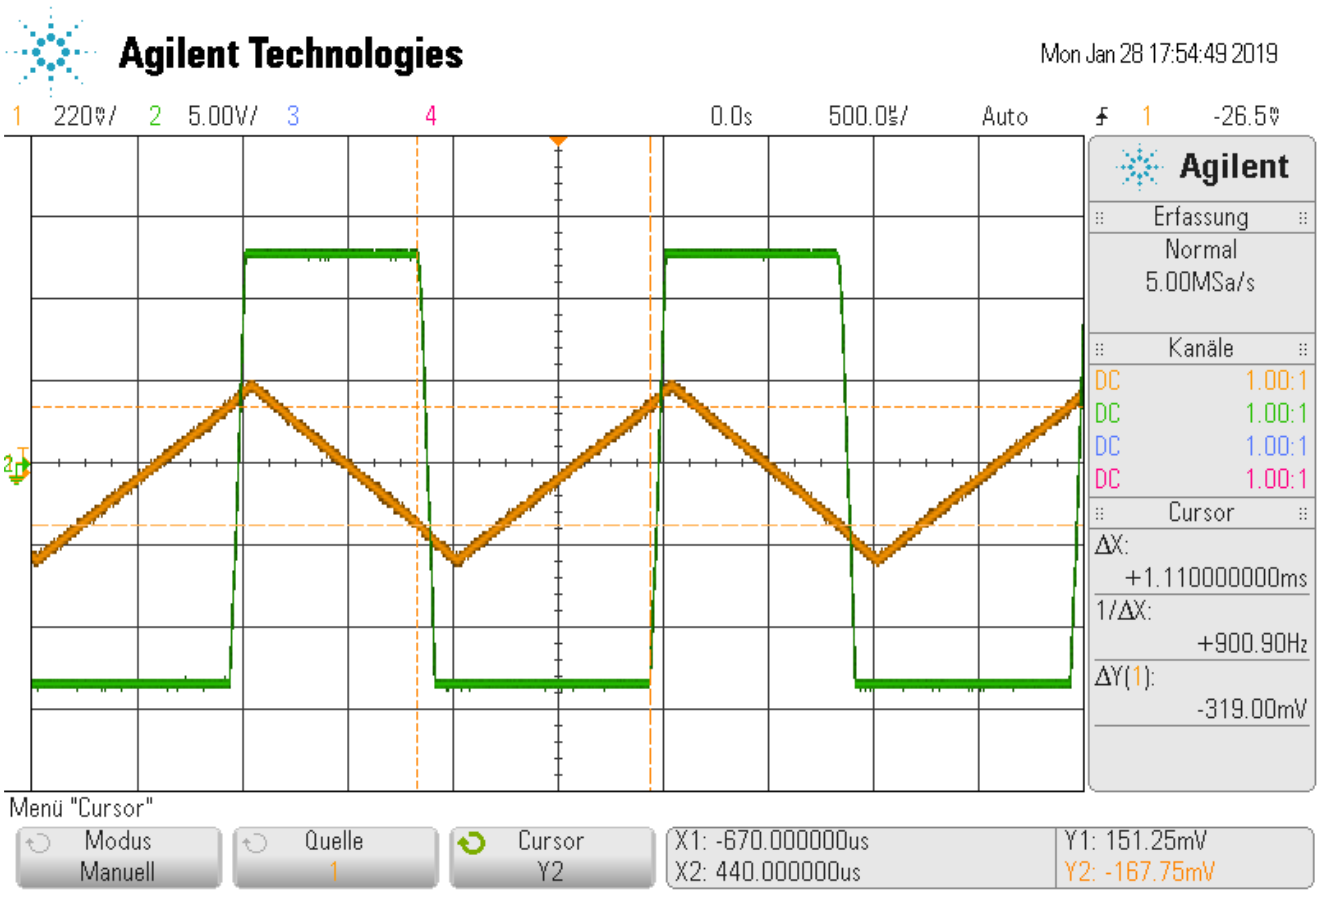
\includegraphics[width=0.7\linewidth]{data_of_others_cuz_ours_suck/schmitt/schmitt_2.png}
    \caption{Oszillographische Aufnahme des Schmitt Triggers bei einem dreieckigen Eingangssignal.}
    \label{fig:schmitt}
\end{figure}
\FloatBarrier
Werden die beiden gemessenen Werte vergleichen ergibt sich eine Abweichung von
0,7\% für die obere Schaltschwelle und 11\% für die untere Schaltschwelle.

\section{Der Signalgenerator \cite{signal}}
Wird hinter dem Schmitt Trigger ein invertierender Integrator geschaltet, lässt sich 
ein Signalgenerator (vgl.\autoref{fig:Signal}) erzeugen. 
Für die im Experiment verwendeten Bauteile gilt $R_1 = \SI{1}{\kilo\ohm}$, $R_2 = \SI{100}{\kilo\ohm}$,
$R_3 = \SI{100}{\kilo\ohm}$ und $C = \SI{1}{\micro\farad}$.\cite{signal}

Da hinter dem Schmitt Trigger ein invertierender Integrator aufgebaut ist, wird eine Dreieckspannung
als Ausgangssignal erwartet.
Das Bild, welches am Oszilloskop aufgenommen worden ist ist in \autoref{fig:Signalgen}
zu sehen.
\begin{figure}
    \centering
    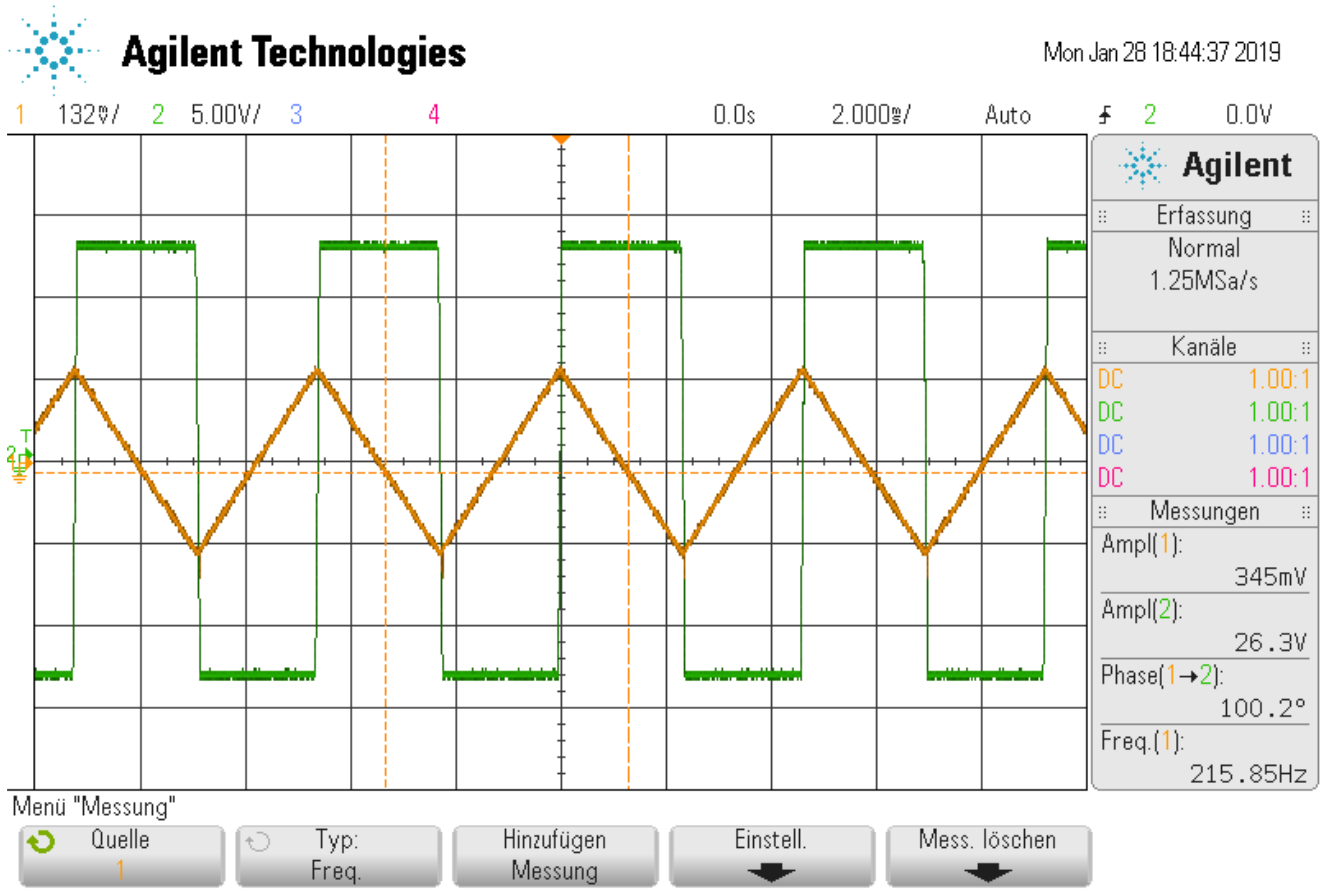
\includegraphics[width=0.7\linewidth]{data_of_others_cuz_ours_suck/Signal/Bildschirmfoto vom 2022-02-11 13-19-10.png}
    \caption{Oszillographische Aufnahme des Signal nach dem Schmitt Trigger (grün) und 
    nach dem invertierenden Integrators. Der orangefarbene Graph ist das Ausgangssignal und die erwartete
    Dreieckspannung.}
    \label{fig:Signalgen}
\end{figure}
\FloatBarrier

Die gemessene Frequenz der Ausgangsspannung beträgt $\SI{216}{\hertz}$.
Verglichen mit dem erwarteten Wert, welcher sich nach
\begin{equation}
    f_\text{Dreieck} =  \frac{R_2}{4 C R_1 R_3} = \SI{250}{\hertz}
\end{equation}
berechnet, ergibt sich eine Abweichung von 14\%.

%
%\begin{equation}\label{eq:xxx}    
%    \begin{split}
%        \lambda &= \SI{855}{\angstrom}\\
%        \delta_\text{ps} &= 0,6\cdot 10^{-6}\\
%        \delta_\text{si}&= 6,8\cdot 10^{-6} \\
%        n_\text{luft} &= 1 \\
%        n_\text{ps} &= 1 - \delta_\text{ps} \\
%        n_\text{si} &= 1 - \delta_\text{ps} 
%    \end{split}
%\end{equation}